\chapter{PLAYER CHARACTER RACES}

\begin{multicols}{2}

\index{Races}All player characters are members of one of six fantasy races including human.  Each race possesses advantages and disadvantages as well as advancement restrictions and ability requirements.  The description for each race is a general description.  Players should not feel bound by the assumptions made in a race's description.

\section{ABILITY SCORE REQUIREMENTS}

All non-human or demi-human races have \index{Ability Scores!Racial Requirements}ability score requirements and maximum limits.  In order for a character to qualify for the race they must meet the base requirement on their ability score rolls.  If the base score is below or above the requirement, the character does not qualify for the race.

\section{ABILITY SCORE ADJUSTMENTS}

Demi-humans have \index{Ability Scores!Racial Adjustments}racial modifiers to their base ability scores.  Even if the adjusted score puts a character below or above their requirement, the player does not have to select a new race.  These adjustments could possibly reduce a score as low as 2 or increase it as high as 19.

\noindent
\begin{minipage}{\columnwidth}

\captionof{table}{Racial Ability Score Adjustments}\label{scoreadjustments}
\noindent
\begin{tabular}{|m{0.45\columnwidth}|m{0.45\columnwidth}|}
\hline
Race			& Adjustments \\
\hline\hline
\rowcolor[gray]{.9}Dwarf		& +1 Con, $-1$ Dex \\
Elf			& +1 Dex, $-1$ Con \\
\rowcolor[gray]{.9}Gnome		& +1 Int, $-1$ Wis \\
Halfling	& +1 Dex, $-1$ Str \\
\hline
\end{tabular}

\end{minipage}

\vspace{10pt}

\section{CLASS RESTRICTIONS AND CLASS LEVEL LIMITS}

\index{Class Restrictions}\index{Level Limits}Demi-humans are restricted in what class they may choose and their maximum level.  This reflects the natural tendencies of a demi-human race and their additional powers.  Humans can choose any class and advance to any level.

\end{multicols}

\noindent
\begin{minipage}{\columnwidth}

\captionof{table}{Demi-human Ability Score Requirements}\label{abilityscorereqs}
\noindent
\begin{tabular}{|m{0.142\textwidth}|m{0.142\textwidth}|m{0.142\textwidth}|m{0.142\textwidth}|m{0.142\textwidth}|m{0.142\textwidth}|}
\hline
Ability			& Dwarf	& Elf	& Gnome	& Half-Elf	& Halfling \\
\hline\hline
\rowcolor[gray]{.9}Strength		& 8/18	& 3/18	& 6/18	& 3/18		& 7/18* \\
Dexterity		& 2/17	& 6/19	& 3/18	& 6/18		& 7/19 \\
\rowcolor[gray]{.9}Constitution	& 11/19	& 7/18	& 8/18	& 6/18		& 10/18 \\
Intelligence	& 3/18	& 8/18	& 6/19	& 4/18		& 6/18 \\
\rowcolor[gray]{.9}Wisdom			& 3/18	& 3/18	& 2/18	& 3/18		& 3/17 \\
Charisma		& 3/17	& 8/18	& 3/18	& 3/18		& 3/18 \\
\hline
\end{tabular}
\noindent
\begin{tabular}{p{\textwidth}}
*Halfling fighters do not gain exceptional strength. \\
\end{tabular}\vspace{.5em}

\end{minipage}

\noindent
\begin{minipage}{\columnwidth}

\captionof{table}{Racial Class Restriction}\label{classrestrictions}
\noindent
\begin{tabular}{|m{0.11\textwidth}|m{0.11\textwidth}|m{0.11\textwidth}|m{0.11\textwidth}|m{0.11\textwidth}|m{0.11\textwidth}|m{0.17\textwidth}|}
\hline
Class		& Human	& Dwarf		& Elf	& Gnome	& Half-Elf	& Halfling \\
\hline\hline
\rowcolor[gray]{.9}Bard		& U		& No		& No	& No	& U			& No \\
Cleric		& U		& 10		& 12	& 9		& 14		& 8 \\
\rowcolor[gray]{.9}Druid		& U		& No		& No	& No	& 9			& No \\
Fighter		& U		& 15		& 12	& 11	& 14		& 9 \\
\rowcolor[gray]{.9}Illusionist	& U		& No		& No	& 15	& No		& No \\
Mage		& U		& No		& 15	& No	& 12		& No \\
\rowcolor[gray]{.9}Paladin		& U		& No		& No	& No	& No		& No \\
Ranger		& U		& No		& 15	& No	& 16		& No \\
\rowcolor[gray]{.9}Thief		& U		& 12		& 12	& 13	& 12		& 15 \\
\hline
\end{tabular}
\noindent
\begin{tabular}{p{\textwidth}}
U Unrestricted advancement. \\
No This race can never advance in the class. \\
\end{tabular}\vspace{.5em}

\end{minipage}

\pagebreak

\begin{multicols}{2}

\section{LANGUAGES}

\index{Languages}Demi-humans begin play knowing common and their native language.  Demi-humans may also know additional bonus languages based on their intelligence but are restricted to the languages listed in their description.  Humans begin play knowing common but are not restricted to their choice of bonus languages.

\noindent
\begin{minipage}{\columnwidth}

\captionof{table}{Player Character Languages}\label{languages}
\noindent
\begin{tabular}{|p{0.3\columnwidth}|p{0.6\columnwidth}|}
\hline
Player Character Languages			& Typical Speakers \\
\hline\hline
\rowcolor[gray]{.9}Common			& Most civilized races \\
Burrow speak*	& Foxes, rabbits, moles, squirrels, burrowing mammals \\
\rowcolor[gray]{.9}Druidic**		& Druids \\
Dwarven			& Dwarves \\
\rowcolor[gray]{.9}Elven			& Elves \\
Giant			& Ogres, giants, trolls \\
\rowcolor[gray]{.9}Goblin			& Goblins, bugbears \\
Gnoll			& Gnolls \\
\rowcolor[gray]{.9}Gnome			& Gnomes \\
Halfling		& Halflings \\
\rowcolor[gray]{.9}Hobgoblin		& Hobgoblins \\
Kobold			& Kobolds \\
\rowcolor[gray]{.9}Orc				& Orcs \\
\hline
\end{tabular}
\noindent
\begin{tabular}{p{\columnwidth}}
* Gnomes only **Druids only \\
\end{tabular}\vspace{.5em}

\end{minipage}

\section{DWARVES}

\index{Dwarf}Dwarves are short, stocky mountain dwelling folk.  They stand on average 4 feet tall with broad shoulders and live to be about 350 years old.  Dwarves have black, brown, red, and platinum blonde hair, dark eyes, and earth tone skin.  Male dwarves pride themselves on their long beards, sometimes styled in braids with decorative features like skulls and gems.  Female dwarves can grow beards but most prefer prominent sideburns or smooth faces.  

Dwarves are typically miners, engineers, warriors and craftsmen that build mighty fortresses in the hills and mountains.  They have a love for metal, gems, and fine drink, often sealing deals with their powerful brews.  Most dwarves are orderly, hierarchal, and believe in strong family bonds with large clans gathering together for mutual protection.  Dwarves are extremely proud of their heritage, quick to anger, wary of strangers, loyal to friends, and slow to forget grudges.

Because of their homes, dwarves are constantly in combat with evil mountain dwelling races including goblinoids, orcs, and some giants.  Dwarves are suspicious of half-orcs who share heritage with their hated enemy orcs.  Elves tend to annoy dwarves, as their aloof and flippant nature is the dwarves' direct opposite.  Dwarves are generally friendly to their distant cousin gnomes who share a love of the earth as well as humans who tend to be dedicated in their work.

\paragraph{Size:} Man-sized.  Although short and stocky, a dwarf's upper body physically resembles a normal man.
 
\paragraph{Classes:} Dwarves can be a cleric, fighter, thief, and multi-class as a fighter/cleric or fighter/thief.

\paragraph{Languages:} Dwarves know common and dwarven.  They may learn gnome, goblin, kobold, orc, and giant.

\end{multicols}

\noindent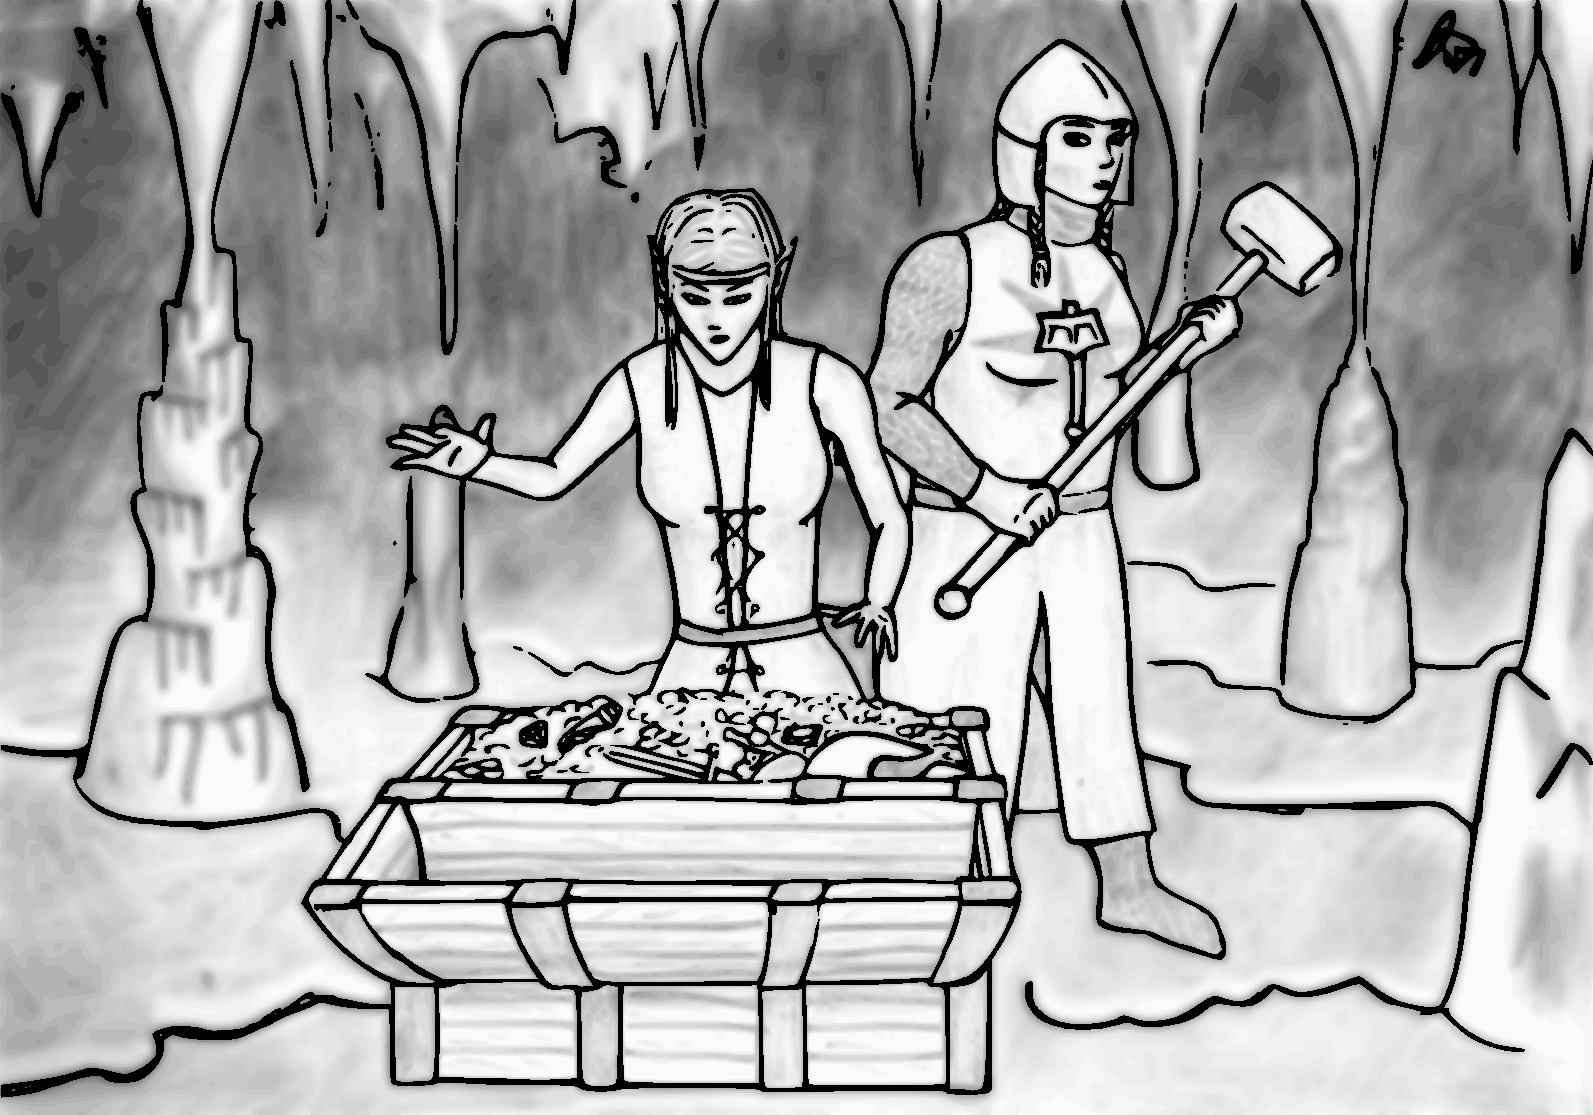
\includegraphics[width=\columnwidth]{treasurefind.pdf}\label{dwarfnelf}

\begin{multicols}{2}

\index{Magic Resistance!Dwarves}\paragraph{Magic Resistant:} Dwarves' non-magical nature gives them a +1 bonus for every 3.5 points of constitution to saving throws vs. wands, staves, rods, and spells.

\index{Poison Resistance!Dwarves}\paragraph{Poison Resistance:} Dwarves receive a +1 bonus for every 3.5 points in constitution to saving throws vs. poison.

\index{Magical Item Malfunction Chance!Dwarves}\paragraph{Magical Item Malfunction:} All magical items used by a dwarf that aren't specific to their class have a 20\% chance of failure.  The dwarf may try again, but that specific activation fails and a charge is spent if applicable.

\index{Favored Enemy!Dwarves}\paragraph{Favored Enemy:} Dwarves receive a +1 bonus on attack rolls against orcs, half-orcs, goblins, and hobgoblins.  

\index{Combat Training!Dwarves}\paragraph{Combat Training:} Ogres, trolls, ogre magi, giants, and titans that attack a dwarf suffer a $-4$ penalty to their attack.  
 
\paragraph{Infravision:} Dwarves have 60-foot infravision.

\index{Stone Cutting!Dwarves}\paragraph{Stone cunning:} Dwarves are naturally cunning when faced with natural stone.  When actively searching within 10 feet of natural stone they may make a special check to detect the following:

Grade or slope in passage: 1--5 on 1d6

New tunnel or passage: 1--5 on 1d6

Sliding/shifting walls or rooms: 1--4 on 1d6

Stone traps and pits: 1--3 on 1d6

Approx. depth underground: 1--3 on 1d6

\paragraph{Ability Score Adjustments:} Dwarves add +1 to their constitution and $-1$ to their charisma.  

\paragraph{Movement Value:} 9

\section{ELVES}

\index{Elf}Elves are a fair, long-lived race standing a foot shorter than the average human and living well over 500 years.  They physically resemble shorter humans with fair skin, pointed ears, smooth faces, black, brown or blonde hair and eyes that range from blue, green, or brown.  Elves grow their hair long and decorate it in intricate designs.  They love loose fitting clothing made of fine silks and fabrics with forest colors like green and red.

Other races view elves as being aloof and apathetic.  Elves are simple folk who care little for the events outside their homes.  They love nature, building their small communes high in the trees or in groves.  Elves value beauty, seeing the artistic intricacies in even the most mundane aspect of nature, and enjoy good music, fine foods, and poetry.

Elves find dwarves boorish and humans impulsive.  Elves get along well with halflings who live peacefully among nature and gnomes who share the elves' love of art and magic.  Despite their attitude, elves are fierce fighters with sword, bow, and magic.  They're forever loyal to friends and wrathful against the evil denizens of nature.  

\paragraph{Classes:} Elves can be a cleric, fighter, mage, thief, or ranger and multi-class as fighter/mage, fighter/thief, fighter/mage/thief, or mage/thief.

\paragraph{Languages:} Elves know elven and common.  They may learn gnome, halfling, goblin, hobgoblin, orc, and gnoll. 

\index{Enchantment Resistance!Elves}\paragraph{Enchantment Resistant:} Elves have 90\% resistance against all sleep and charm spells. 

\index{Expert Pull!Elves}\paragraph{Expert Pull:} When using bows (but not crossbows), elves get a +1 bonus to attack rolls.

\index{Sword Expertise!Elves}\paragraph{Sword Expertise:} When using short or long swords, elves get a +1 bonus to attack rolls.

\index{Stealth!Elves}\paragraph{Stealthy:} An elf imposes a $-4$ penalty to surprise rolls against opponents.  This bonus only applies if the elf isn't wearing metal armor, is alone or with a group entirely composed of elves and/or halflings, or the elf is further than 90 feet from his traveling group.  When performing a complicated physical task such as opening a door or climbing, the applied penalty is $-2$. 

\paragraph{Infravision:} Elves have infravision out to 60 feet.

\index{Keen Senses!Elves}\paragraph{Keen Senses:} Elves have a natural tendency to notice secret or concealed door merely by passing within 10 feet.

Secret or concealed door: 1 on 1d6

Secret door (searching): 1--2 on 1d6

Concealed door (searching): 1--3 on 1d6

\paragraph{Ability Score Adjustments:} Elves receive a +1 bonus to dexterity and a $-1$ penalty to constitution.  

\paragraph{Movement Value:} 12

\section{GNOMES}

\index{Gnome}Gnomes are distant cousins of dwarves that live in remote regions far from civilization.  They're smaller, thinner in frame, with darker earth colored skin and bulbous noses.  Gnomes wear their hair short and males keep their beards short and stylized.  Gnomes wear simple garb and are fond of gems of all sorts.

Gnomes live in hilly or heavily forested areas untouched by man.  They live in small communities where they fish, weave, and cultivate herbs.  Gnomes are expert gem cutters, love good music, and enjoy harmless practical jokes.  Being less reserved than dwarves, gnomes are highly inquisitive and curious to a fault.   

Gnomes are indifferent yet inviting to all peaceful races but are friendly with their dwarven cousins.  Gnomes are friendly with woodland creatures, pixies, brownies, and other fey.  A gnomish adventurer seeks to experience the wide and wondrous world outside his burrow.

\paragraph{Size:} Small.  Small creatures must wear specially crafted armor and require two hands to wield man-sized weapons.

\paragraph{Classes:} Gnomes can be a fighter, thief, cleric, or illusionist.  Gnomes can multi-class as fighter/thief, fighter/cleric, fighter/illusionist, thief/cleric, thief/illusionist, and cleric/illusionist.  

\paragraph{Languages:} Gnomes know common and gnome.  They may learn dwarf, halfling, goblin, kobold, and burrow speak, a language of chirps, clicks, and body motion used to speak with burrowing mammals such as badgers, moles, foxes, groundhogs, weasels, and rabbits.  Because animals have limited intelligence, only basic things like emotion, simple objects, and locations can be communicated clearly.

\index{Magic Resistance!Gnomes}\paragraph{Magic Resistant:} Gnomes receive a +1 bonus for every 3.5 points of constitution on saving throws vs. wands, staves, rods, and spells.

\index{Magic Item Malfunction Chance!Gnomes}\paragraph{Magic Item Malfunction:} Gnomes have a 20\% malfunction chance when activating any magical item that's not a weapon, armor, shield, illusionist item, or if the gnome is also a thief, items that duplicate thieving abilities.  Failure indicates the item doesn't activate but a charge is spent.

\index{Favored Enemy!Gnomes}\paragraph{Favored Enemy:} Gnomes gain a +1 bonus to attack rolls against kobolds and goblins. 

\columnbreak

\noindent
\includegraphics[width=\columnwidth, height=9.25in]{testblock.pdf}  
 
\index{Combat Training!Gnomes}\paragraph{Combat Training:} Gnomes apply a $-4$ penalty to attack rolls when attacked by gnolls, bugbears, ogres, trolls, ogre magi, giants, and titans.  

\paragraph{Infravision:} Gnomes have 60-foot infravision.

\index{Stone Cutting!Gnomes}\paragraph{Stone cunning:} Gnomes can detect special properties of natural underground spaces whenever they're within 10 feet.  Gnomes must actively concentrate to detect the following:

Incline or slope: 1--5 on 1d6

Unstable walls, ceiling, or floor: 1--7 on 1d10

Approx. depth underground: 1--4 on 1d6

Direction underground: 1--3 on 1d6

\paragraph{Ability Score Adjustment:} Gnomes receive a +1 bonus to intelligence and a $-1$ penalty to wisdom.

\paragraph{Movement Value:} 6

\section{HALF-ELVES}

\index{Half-elf}Half-elves are an interspecies mix of human and elf, combining aspects of both races and living about twice as long as a human.  Physically they resemble elves although taller, heavier and with a less exaggerated taper in their ears.  Male half-elves can grow beards like a human but they prefer short, trimmed facial hair and neatly styled hair.  Half-elves adopt the clothing, culture, and personality of the community they live in.

Half-elves form no specific communities of their own; rather, they're found among humans or elves, and generally accepted into society.  In less civilized areas, humans and elves treat half-elves with racism and bigotry.  In some areas, a half-elf is viewed as a mediator between races.  Because of their openness, charisma, and willingness to feel accepted, half-elves make ideal diplomats and bards.

\paragraph{Classes:} Half-elves can be a cleric, druid, fighter, ranger, mage, wizard, thief, or bard.  A half-elf can multi-class as cleric/fighter, druid/fighter, cleric/fighter/mage, druid/fighter/mage, cleric/ranger, druid/ranger, cleric/mage, druid/mage, fighter/mage, fighter/thief, fighter/mage/thief, or mage/thief.  

\paragraph{Languages:} Half-elves know common and elven.  They may learn gnome, halfling, goblin, hobgoblin, orc, and gnoll.  

\index{Enchantment Resistance!Half-elves}\paragraph{Enchantment Resistance:} Half-elves have a 30\% resistance to sleep and charm related spells.

\paragraph{Infravision:} Half-elves have 60-foot infravision.

\index{Keen Senses!Half-elves}\paragraph{Keen Senses:} Half-elves have a natural tendency to notice secret or concealed door merely by passing within 10 feet.

Secret or concealed door: 1 on 1d6

Secret door (searching): 1--2 on 1d6

Concealed door (searching): 1--3 on 1d6

\paragraph{Movement Value:} 12

\section{HALFLINGS}

\index{Halfling}Halflings are a small, slightly rotund people physically looking like short humans.  They have human hair and eye tones, plump faces, rosy complexion, and rarely grow facial hair.  Halflings have large, powerful feet (males grow coarse hair on top) and usually avoid wearing boots as constructing them for their size is difficult.  

Halflings live in simple towns, are industrious, but not overly dedicated, and enjoy the company of others.  Halflings prefer the comforts of home to adventuring and value tales of the outside world over leaving their well-furnished burrows.  Halflings aren't apathetic, but they're motivated by anything that makes their life more comfortable.  They're not cowardly, but they would sooner avoid a fight than engage in one.

Halflings get along well with all races.  Elves view them as cheerful simpletons.  Dwarves tolerate their good nature.  Gnomes prefer halfling company and hospitality.  The taller races tend to be suspicious of halflings as their short size makes them quintessential pickpockets.  

\paragraph{Size:} Small.  Small creatures must wear specially crafted armor and require two hands to wield man-sized weapons.

\paragraph{Classes:} Halflings may be a cleric, fighter, thief, or multi-class as a fighter/thief.  

\paragraph{Languages:} Halflings know common and halfling.  They may learn dwarf, elf, gnome, goblin, and orc.

\index{Magic Resistance!Halflings}\paragraph{Magic Resistance:} Halflings receive a +1 bonus for every 3.5 points in constitution on saving throws against wands, staves, rods, and spells.

\index{Poison Resistance!Halflings}\paragraph{Poison Resistance:} Halflings gain a bonus to saving throws vs. poison equal to +1 for every 3.5 points in constitution.

\index{Sling Training!Halflings}\paragraph{Sling Training:} Halflings receive a +1 bonus on attack rolls when using a hurled weapon or sling.

\index{Stealth!Halflings}\paragraph{Stealthy:} Halflings impose a $-4$ penalty to surprise rolls against opponents.  This bonus only applies if the halfling isn't wearing metal armor, is alone or with a group entirely composed of halflings and/or elves, or the halfling is further than 90 feet from his traveling group.  When performing a complicated physical task such as opening a door or climbing, the applied penalty is $-2$.

\paragraph{Infravision:} Halflings have 60-foot infravision.

\index{Nature Cunning!Halflings}\paragraph{Nature Cunning:} Halflings can assess information about their natural surroundings.  The halfling must concentrate for at least one round before making a check.

Detect up or down slope: 1--3 on 1d4

Discern direction: 1--3 on 1d6

\paragraph{Ability Score Adjustments:} Halflings receive a +1 bonus to dexterity and a $-1$ penalty to strength.

\paragraph{Movement Value:} 6

\section{HUMANS}

\index{Human}In game terms, human is an all-encompassing race; however they're as diverse and varied as the humans in the real world.  Because humans are more dedicated and driven than other races, humans have no class restrictions.  Humans in general are more tolerant of other races and humans are found among any race that accepts them.  Because of their high birth rate, quick maturation compared to other races, industrious attitude, tenacity, and ingenuity, humans have created vast empires and spread their influence to every corner of the world.

\paragraph{Classes:} Any

\paragraph{Languages:} Common.  Humans may learn any language they would reasonably have access to.

\paragraph{Movement Value:} 12

\end{multicols}

\noindent
\includegraphics[width=\columnwidth, height=4.5in]{testblock.pdf}  

\begin{multicols}{2}

\section{HEIGHT, WEIGHT, AND AGE}

\index{Age}\index{Height and Weight}After assigning ability scores and choosing a race and gender, the player should choose his character's height, weight, and age or roll for them randomly.  \index{Ability Scores!Aging Effects}Age has effects on a character's ability scores.  There are three steps to aging; middle, old, and venerable.  Each step provides a cumulative penalty to physical ability scores and a bonus to mental scores.  The GM secretly rolls a variable to determine the maximum age of a specific character.

Some effects magically age a character.  Characters do not gain the mental bonuses of magical aging but do gain the penalties applied.  Effects that reduce a characters age likewise removes the physical penalties but not the mental bonuses.

\end{multicols}

%\newpage

\noindent
\begin{minipage}{\columnwidth}

\captionof{table}{Height and Weight}\label{heightweight}
\noindent
\begin{tabular}{|m{0.176\textwidth}|m{0.176\textwidth}|m{0.176\textwidth}|m{0.176\textwidth}|m{0.176\textwidth}|}
\hline
Race		& Base Height		& Modifier	& Base Weight	& Modifier \\
\hline\hline
\rowcolor[gray]{.9}Dwarf		& 43"/41"			& 1d10		& 130 lbs./105 lbs.		& 4d10 \\
Elf			& 55"/50"			& 1d10		& 90 lbs./70 lbs.		& 3d10 \\
\rowcolor[gray]{.9}Gnome		& 38"/36"			& 1d6		& 72 lbs./68 lbs.		& 5d4 \\
Half-elf	& 60"/58"			& 2d6		& 110 lbs./85 lbs.		& 3d12 \\
\rowcolor[gray]{.9}Halfling	& 32"/30"			& 2d8		& 52 lbs./48 lbs.		& 5d4 \\
Human		& 60"/59"			& 2d10		& 140 lbs./100 lbs.		& 6d10 \\
\hline
\end{tabular}

\end{minipage}

\noindent
\begin{minipage}{\columnwidth}

\captionof{table}{Age}\label{age}
\noindent
\begin{tabular}{|m{0.11\textwidth}|m{0.11\textwidth}|m{0.11\textwidth}|m{0.11\textwidth}|m{0.11\textwidth}|m{0.11\textwidth}|m{0.17\textwidth}|}
\hline
Race	& Starting Age	& Variable	& Max Age	& Middle Age*	& Old Age** & Venerable*** \\
\hline\hline
\rowcolor[gray]{.9}Dwarf		& 40	& 5d6	& 250~+~2d100	& 125	& 167	& 250 \\
Elf			& 100	& 5d6	& 350~+~4d100	& 175	& 233	& 350 \\
\rowcolor[gray]{.9}Gnome		& 60	& 3d12	& 200~+~3d100	& 100	& 133	& 200 \\
Half-elf	& 15	& 1d6	& 125~+~3d20	& 62	& 83	& 125 \\
\rowcolor[gray]{.9}Halfling	& 20	& 3d4	& 100~+~1d100	& 50	& 67	& 100 \\
Human		& 15		& 1d4	& 90~+~2d20	& 45	& 60	& 90 \\
\hline
\end{tabular}
\noindent
\begin{tabular}{p{\textwidth}}
*$-1$ Str/Con; +1 Int/Wis \\
** $-2$ Str/Dex, $-1$ Con; +1 Wis \\
*** $-1$ Str/Dex/Con; +1 Int/Wis \\
\end{tabular}\vspace{.5em}

\end{minipage}

